%-----------------------------------------------------------------------------------%
\section{Introduction\label{sec:intro2dm}}
%-----------------------------------------------------------------------------------%

I'll attempt to explain the dark matter problem at an entry level with the following thought experiment.
Let's say you're the teacher for an elementary school classroom.
You take them on a field trip to your local science museum and among exhibits is one for mass and weight.
The exhibit has a gigantic scale, and you come up with a fun problem for your classroom.

You say to your class, "What is the total weight of the classroom?
Give your best estimation to me in 30 minutes, and then we'll check on the scale.
If your guess is within 10\% of the right answer, we will stop for ice cream on the way back"

The students are ecstactic to hear this, and they get to work.
The solution is some variation of the following strategy.
The students should give each other their weight or best guess if they don't know.
Then, all they have to do is add each students' weight and get a grand total for the class.
The measurement on the giant scale should show the true weight of the class.
When comparing the measured weight, multiply the observation by 1.1 and 0.9 in order to get the +/- 10\% tolerance respectively.

Two of your students, Sandra and Mario, return to you with a solution.

They say, "We weren't sure of everyone's weight.
We used 65 lbs for the people we didn't know and added everyone who does know.
There are 30 of us, and we got 2,000 lbs!
That's a ton!"

You estimated 1,900 lbs assuming the average weight of a student in your class was 60 lbs.
So you're pleased with Sandra's and Mario's answer.
You instruct your students to all gather on the giant scale and read off the weight together.
To all of your surprise, the scale reads \textit{10,000 lbs}!
10,000 is significantly more than a 10\% error from 2,000.
In fact, it is approximately 5 times more massive than either your or your students' estimates.
You think to yourself and conclude there must be something wrong with the scale.
You ask an employee to check the scale and verify it is calibrated well.
They confirm that the scale is in working order.
You weigh a couple of students individually to test that the scale is well calibrated.
Sandra weighs 59 lbs, and Mario weighs 62 lbs, typical weights for their age.
You then weigh each student individually and see that their weights individually do not deviate greatly from 60 lbs.
So, where does all the extra weight come from?

This thought experiment serves as an analogy to the Dark Matter problem.
The important substitution to make however is to replace the students with stars and classroom with a galaxy, say the Milky Way.
Individually the mass of stars is well measured and defined with the Sun as our nearest test case.
However, when we set out to measure the mass of a collection of stars as large as galaxies, our well motivated estimation is wildly incorrect.
There simply is not way to account for this discrepancy except without some unseen, or dark, contribution to mass and matter in galaxies.
I set out in my thesis to narrow the possibilities of what this Dark Matter could be.

This chapter is organized like the following\dots
\todo{Text should look like ... Chaper x has blah blah blah.}

%-----------------------------------------------------------------------------------%
\section{Dark Matter Basics\label{sec:basicDM}}
%-----------------------------------------------------------------------------------%

Presently, the most compelling Dark Matter (DM) model is $\Lambda$ \textbf{C}old \textbf{D}ark \textbf{M}atter, or \lcdm.
I present the evidence supporting \lcdm~in \ref{sec:evidence4dm}, yet discuss the conclusions of the \lcdm~model here.
According to \lcdm~fit to observations on the Cosmic Microwave Background (CMB), DM is 26.8\% of the universe's current energy budget
Baryonic matter, stuff like atoms, gas, and stars, contributes to 4.9\% of the universe's current energy budget \cite{Greene:cosmology_dm,Young:cosmology_dm,Bertone:particleDM}.

% A note on the above, the number is usually quoted as some \Omega_{f} h^_2. In order to get the percentages yourself, you need to actually multiply h which is the hubble expansion rate.

DM is dark; it doesn't interact readily with light at any wavelength.
DM also doesn't interact noticably with the other standard model forces (Strong and Weak) at a rate that is readily observed \cite{Bertone:particleDM}.
DM is cold, which is to say that the average velocity of DM is below relativisic speeds \cite{Greene:cosmology_dm}.
'Hot' DM would not likely manifest the dense structures we observe like galaxies, and instead would produce much more diffuse galaxies than what is observed \cite{Bertone:particleDM,Greene:cosmology_dm}.
DM is old; it played a critical role in the formation of the universe and the structures within it \cite{Greene:cosmology_dm,Young:cosmology_dm}.

Observations of DM has so far been only gravitational.
The parameter space available to what DM could be therefore is very broad.
Searches for DM are summarized by supposing a hypothesis that has not yet been ruled out, and performing measurements to test them.
When the observations yield a null result, the parameter space is further constrained.
I present some approaches for DM searches in \cref{sec:dm_search}.

%-----------------------------------------------------------------------------------%
\section{Evidence for Dark Matter}\label{sec:evidence4dm}
%-----------------------------------------------------------------------------------%

Dark Matter (DM) has been a looming problem in physics for almost 100 years.
Anomolies have been observed in galactic dynamics as early as 1933 when Fritz Zwicky noticed unusually large velocity dispersions in the Coma cluster.
Zwicky's measurement was the first recorded to use the Virial theorem to measure the mass fraction of visible and invisible matter in celestial bodies~\cite{Hooper:DMHistory}.
From Zwicky in \cite{Zwicky:1933}, "\textit{If this would be confirmed, we would get the surprising result that dark matter is present in much greater amount than luminous matter.}"
Zwicky's and other's observation did not instigate a crisis in astrophysics because the measurements did not entirely conflict with their understanding of galaxies \cite{Hooper:DMHistory}.
In 1978, Rubin, Ford, and Norbert measured rotation curves for ten spiral galaxies \cite{Rubin:1978}.
Rubin et. al.'s 1978 publication presented a major challenge to the conventional understanding of galaxies that could no longer be accreditted to measurement uncertainties.
Evidence has been mounting ever since for this exotic form of matter.
The following subsections sample some of the compelling evidence supporting DM.

%$$$$$$$$$$$$$$$$$$$$$$$$$$$$$$$$$$$$$$$$$$$$$$$$$$$$$$$$$$$$$$$$$$$$$$$$$$$$$$$$$$$%
\subsection{First Clues: Stellar Velocities\label{sec:ev4dm_stars}}
%$$$$$$$$$$$$$$$$$$$$$$$$$$$$$$$$$$$$$$$$$$$$$$$$$$$$$$$$$$$$$$$$$$$$$$$$$$$$$$$$$$$%

Zwicky's, and later Rubin's, measurement of the stellar velocities were built upon the Virial theorem, shown as \virialtheorem
Where \textit{T} is the kinetic energy and \textit{V} is the potential energy in a self-gravitating system.
The potential was defined as the classical Netwon's law of gravity from stars and gas contained in the observed galaxies \newtongravity
Zwicky et. al. measured just the velocities of stars apparent in optical wavelengths \cite{Zwicky:1933}.
Rubin et. al. added by measuring the velocity of the hydrogen gas via the 21 cm emmission line of Hydrogen \cite{Rubin:1978}.
The velocities of the stars and gas are used to infer the total mass of galaxies and galaxy clusters via \cref{eq:virialtheorem}.
An inferred mass is also made from the luminosity of the selected sources.
The two inferences are compared to each other as a luminosity to mass ratio and typically yields \cite{Greene:cosmology_dm}\masslightratio
$M_{\sun}$ and $L_{\sun}$ referring to stellar mass and stellar luminosity respectively.
These ratios clearly indicate a discrepancy in apparent light and mass from stars and gas and their velocities.

Rubin et.al. \cite{Rubin:1978} demonstrated that the discrepancy was unlikely to be an under-estimation of the mass of the stars and gas.
The inferred 'dark' mass was up to 5 times more than the luminous mass.
This dark mass also needed to extend well beyond the extent of the luminous matter.

\begin{figure}[h]
    \centering{
    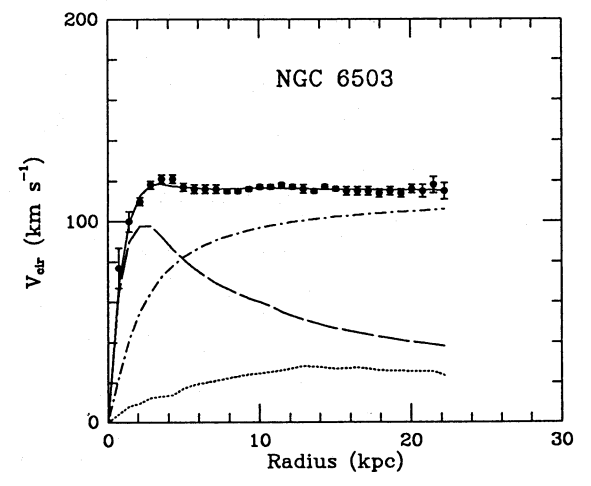
\includegraphics[scale=0.8]{figures/NGC6503_rotcurve.png}
    \caption{Rotation curve fit to NGC 6503 from \cite{Begeman:rot_curves}. Dashed line is the contribution from visible matter. Dotted curves are from gas. Dash-dot curves are from dark matter (DM). Solid line is the composite contribution from all matter and DM sources. Data are indicated with bold dots with error bars. Data agree strongly with matter + DM composite prediction}
    \label{fig:gal_rot_curve}
    }
\end{figure}

\cref{fig:gal_rot_curve}: features one of many observations made on the stellar velocities within galaxies.
The measured roation curves mostly feature a flattening of velocities at higher radius which is not expected if the gravity was only coming from gas and luminous matter.
The extension of the flat velocity region also indicates that the DM is distributed far from the center of the galaxy.
Modern velocity measurements include significantly larger objects, galactic clusters, and smaller objects, dwarf galaxies.
Yet, measurements along this regime are leveraging the virial theorem with Newtonian potential energies.
We know Netwonian gravity is not a comprehensive description of gravity.
New observational techniques have been developed since 1978, and those are discussed in the following sections.

%$$$$$$$$$$$$$$$$$$$$$$$$$$$$$$$$$$$$$$$$$$$$$$$$$$$$$$$$$$$$$$$$$$$$$$$$$$$$$$$$$$$%
\subsection{Mounting Evidence for Dark Matter\label{sec:ev4dm_more}}
%$$$$$$$$$$$$$$$$$$$$$$$$$$$$$$$$$$$$$$$$$$$$$$$$$$$$$$$$$$$$$$$$$$$$$$$$$$$$$$$$$$$%

Modern evidence for dark matter comes from new avenues beyond stellar velocities.
Gravitational micro-lensing from DM is a new channel from general relativity.
The Cosmic Microwave Background shows that the universe had DM in it from a very early stage.
Computational resources have expanded greatly in recent decades enabling universe models that again support the need for DM in the evolution of the universe.

General relativity predicts abberations in light caused by massive objects.
In recent decades we have been able to measure the lensing effects from compact objects and DM haloes.
\cref{fig:grav_lensing_explained} shows how different compact bodies change the final image of a far away galaxy resulting from gravitational lensing.
Gravitational lensing developed our understanding of dark matter in two important ways.

\begin{figure}[h!]
    \centering{
        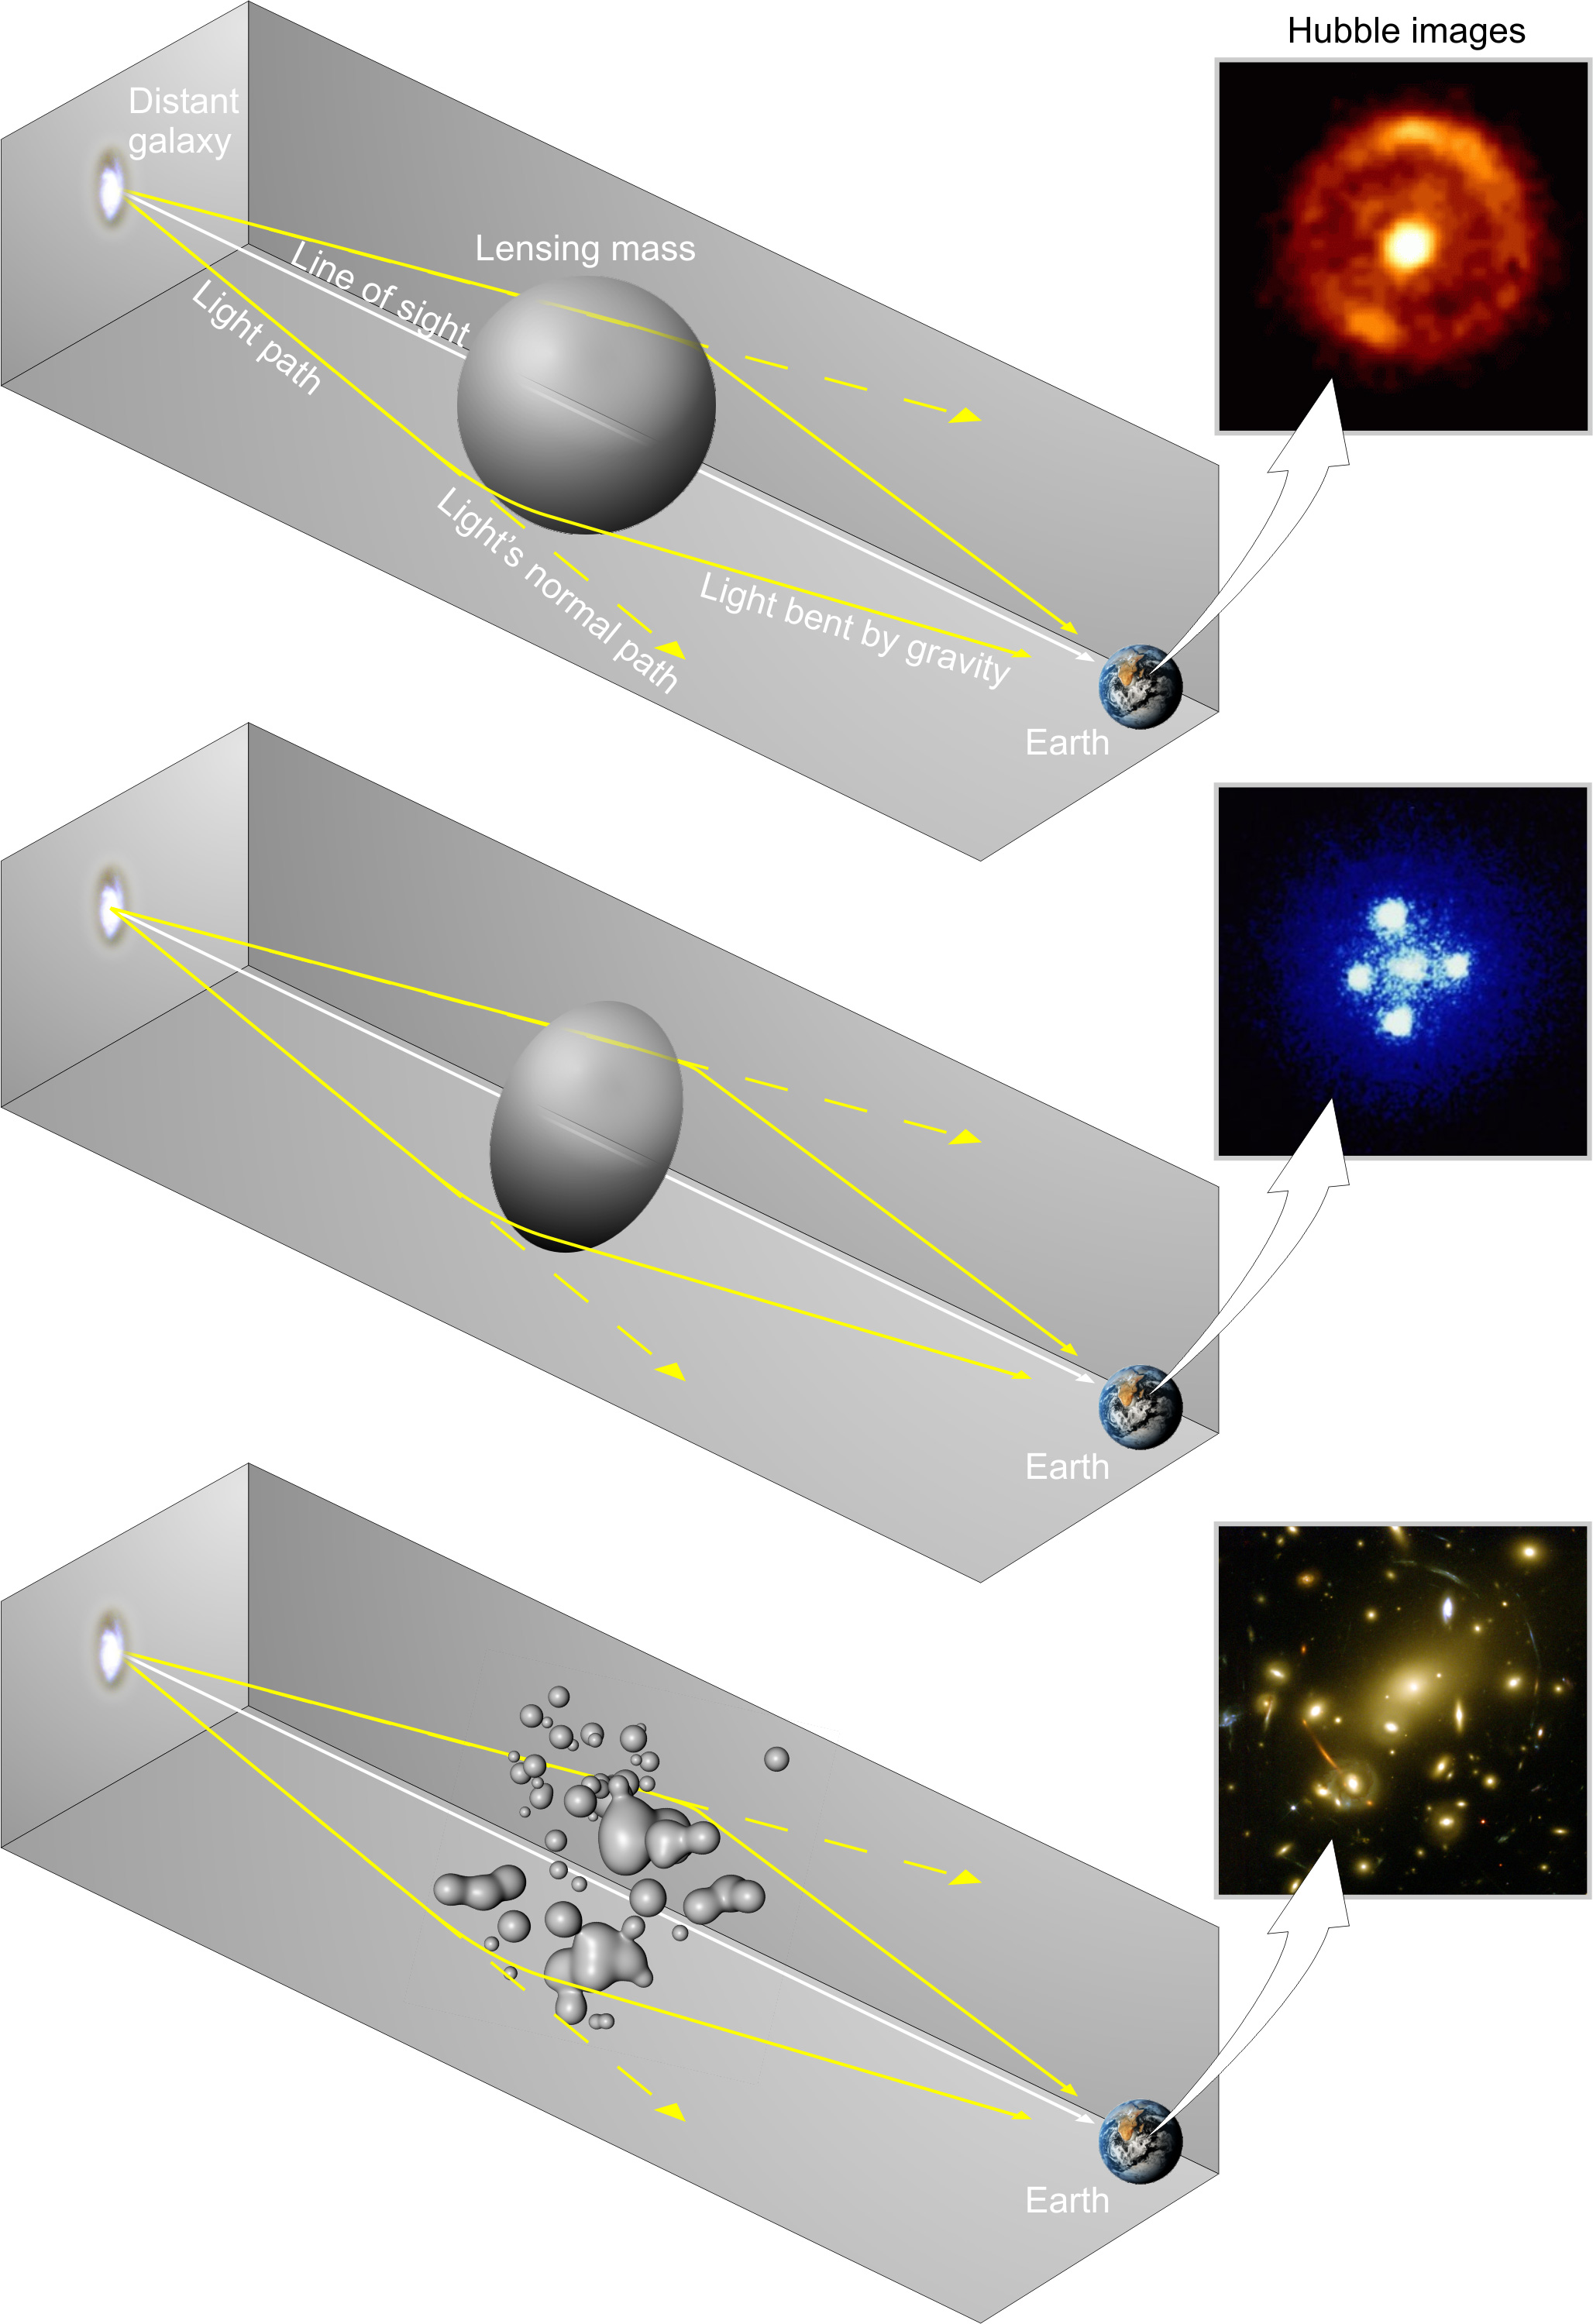
\includegraphics[scale=0.19]{figures/heic0404b.jpg}
        \caption{Light from distant galaxy is bent in different way depending on the distribution of mass between the galaxy and Earth. Yellow dashed lines indicate where the light would have gone if the matter was not present.}
        \label{fig:grav_lensing_explained}
    }
\end{figure}

First, micro-lensing observations, or the lack of them, of our Milky Way halo resulted in a conspicuous absence of massive astrophysical compact halo objects (MACHOs).
The hypothesis was that 'dark matter' could be accounted for by sufficiently dim compact objects.
Such objects include things like planets, brown dwarves, black holes, or neutron stars.
Whenever these objects passed in front of a large luminous source, such as the Large Magelenic Clouds, a variation in light should be observed \cite{Hooper:DMHistory}.
The MACHO and EROS collaborations performed this observation and did not find a substantial contribution to the DM Milky Way halo from MACHOs.
They measured that MACHOs of mass range 0.15 to 0.9 $M_{\sun}$ contributes to an upper limit of 8\% of the DM halo mass \cite{Tisserand:MACHO}.

\begin{figure}[ht]
    \centering{
        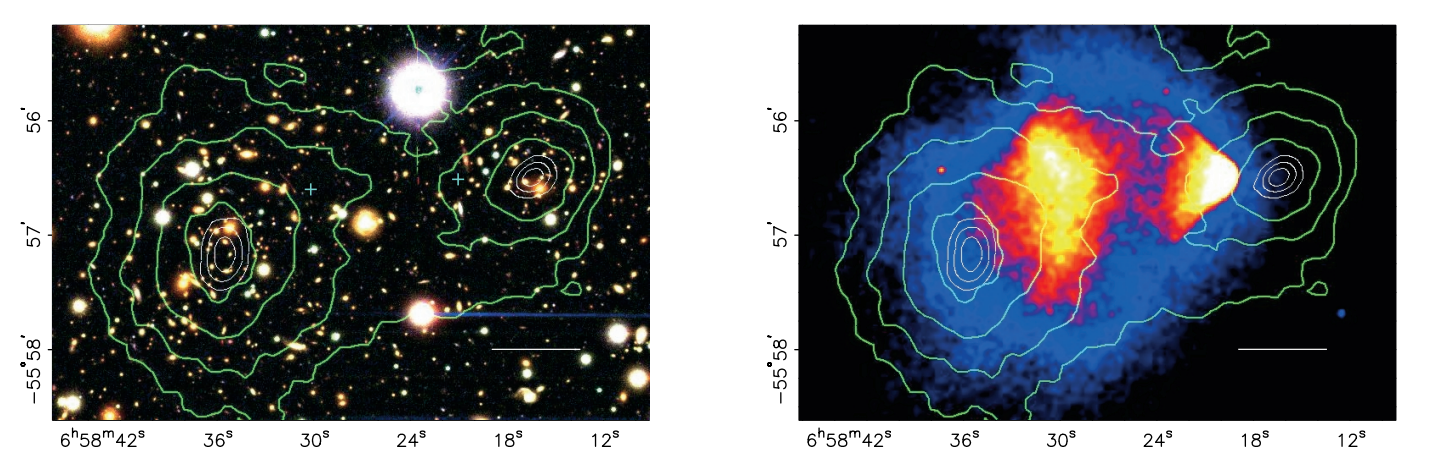
\includegraphics[scale=0.425]{figures/bullet_cluster.png}
        \caption{Woooow}
        \label{fig:bullet_cluster}
    }
\end{figure}

Gravitational lensing can also be applied towards galaxy clusters for DM searches.
The observation of two merging galactic clusters in 2006 provided a compelling arguement for particle DM outside the Standard Model.
These clusters merged recently in astrophysical time scales.
As a result fo the they're recent merge, the stars and galaxies are separated from the intergalactic gas.
For these clusters, the hot, intergalactic gas is responsible for most of the mass in the systems \cite{Hooper:DMHistory}.
The hot gas emits x-rays we observe at Earth.

passed through each other at some point in the past and are in the process of merging \ns.
Two observations of the clusters were made independantly of each other.
The first was the microlensing of light around the galaxies due to their gravitational influences.
When celestial bodies are large enough, the gravity they exert bends space and time itself.
This bending effects light and will deflect light in a smilar way to how lenses will bend light.


With a sufficient understanding of light sources behind a celestial body, you can reconstruct the countours of the gravitational lenses.
The gradient of the contours then tells you how dense the matter is and where it is.

They then made measurements of the x-ray emmision from the clusters.
The idea is that since these galaxies are mostly gass and are merging, then they should be getting hotter.
If they're merging, the x-ray emmisions should be the strongest where the gas is mostly moving through each other.
The x-rays basically map out where the gas is in these merging galaxies.

\tmpfig{bullet cluster photo.}

The dope super interesting thing is that the map of the x-ray emmisions totally doesnt align with the gravitational countours from the microlensing.
This incongruence is really telling that there is a lot of matter somewhere that we jsut cannot see.
Moreover this matter is NOT BARYONIC.
So then what is it?
This measurement didn't really tell us what exactly, but it did suggest that this DM also doesn't interact with itself very strongly.
If it did, then it would have been more aligned with where the x-ray emmision was.
There's been other studies of galaxies with similar results altho there are a handful that resemble something we expect for strongly self-interacting DM. \ns.
This result really makes it hard to argue that DM is somehow something amiss in our gravitational theories.

The CMB is the primordial light from the young universe.
Basically a baby photo.
Then we look at how the simulated universes look like compared to what we see.
From those simulations we infer how much dark matter is in the universe.
The fuller explinations and shortcoming of each of these methods is explained further in this section.

we got the CMB and geometry of the universe.
So there's this thing called the cosmic Microwave Background (CMB).
It's the universes baby photo from when all of the hydrogen de-ionized to form atoms.
This happened cause it was cold enough finally from the expansion of the universe.
The recombination happened someitme around less than 1 mil years after the universe was born \fu \ns.
when hydrogen absorbs an electron, it releases a photon of a specific wavelength.
This wavelength amounts to 13 ev or so according to the qm eqn\dots

\eqin{hydrogen energy level}

However the universe has been expnding since it's creation.
In fact the time and space itself is exanding away from us for as long as the universe is old.
This red-shifts the combination light into the Microwave frequencies.
This is the light we can detect with microwave observatories and is what was first detected by so and so in the 19?? \ns \fu
This make a microwave image seen below after we subtract the average of the image.

\tmpfig{CMB photo}

We can do a funny thing with the photo but it's fairly straight forward.
Shove the photo into a spherical harmonic decomposition.
This gives you the vibrational modes of the CMB and therefore the early universe.
The important thing to note is that the harmoincs are based on primordial baryonic acoustic oscillations \fu
This is directly linked with the energy density of the universe and how these couple.
It's a cosmology and geometry thing.

\tmpfig{Planl harmonics of CMB}

The harmnics would look very different for a universe with less dmm (see fig bla) or a lot more dm (see fig bla)

\tmpfig{Plank harmonics vs DM content CMB}

The observations fit well with the Lambda CDM model and we derive the primordial dm concentration to be XX\% and primordial DM to be XX\%.
\todo{What are the shortcomings?} I think the most obcious arguement is simply that this is very old light, up to 13.6 billion years old.
It's not at all necessary that the universe shares the exact same DM, matter ratio.
There is a poorness in fit in the lower region of the graph and this is unexplained.
The way we measure distance can be really fucked sometimes so maybe that's a problem too.

Finally we have universe simulations like the millenium simultation and more \fu \ns.
These are computer simulations of the unverse with different fractions of DM and baryonic matters.
Additionaly hypotheses are tested like how hot the DM is and how strongly it interacts with itself and with baryonic matter.
These simulations are also done for smaller scales like galactic formation and galaxy clustering.
In alls cases the simulations most resemble out universe for a Lambda CDM like universe.

The main issues with the similations is mostly that we cant perfectly simulate the unverse.
They are often imcomplete with how they treat baryonic matter and make big assumptions about dark matter.
These simulations also have to contend with very real computational limitations.
The resultion of some of the universe simulations are as large at XX's of solar masses.
There's reason to beleive that the resultion might really matter as well. \ns \fu


Overall this forms a compelling arguement for dark matter.
However, these observations really only confirm that DM is there.
It takes another leap of theory to make observations of DM that are nongravitational.
One of which is the emergence of the Weakly Interacting Massive Particle hypothesis of DM.
This DM candidate theory is discussed futher in the next section.

%-----------------------------------------------------------------------------------%
\section{Searching for Dark Matter}\label{sec:dm_search}
%-----------------------------------------------------------------------------------%
We've explored any options for what dark matter could be now.
The remainder of this thesis I will focus only on a particle dark matter hypothesis.
I will not be discussin alternative gravitational theories such as Modified Newtonian Dynamics.
I am also ignoring composite dark matter discussion like primordial black holes, dark atoms, or dark bound states of baryonic matter.
For this thesis I focus on the hypothesis that DM is a weakly interacting and massive particle (WIMP).

\tmpfig{Standard model. Square or Circle?}

The current status of the standard model does not have a WIMP candidate.
When looking at the standard model, we can immediately exclude any charged particle.
This is because charged particles interact with light and so much DM would be immediately visible if is had the same charge as SM particles.
Specifically this will rule out the following charged, fundamental particles: $e,\mu, \tau, W, u, d, s, c, t, b$ and their corresponding antiparticles.
Recalling from earlier that DM must be long lived and stable over the age of the universe.
This would exclude all SM particles with decay half-lives at or shorter than the age of the universe.
This constraint eliminates the $Z, $and $H$ bosons.
Finally, the candidate DM needs to be somewhat massive.
This follows from the DM needing to be cold or not relativistic through the universe.
This eliminates the remaining SM particles: $\nu_{e, \mu, \tau}, g, \gamma$.
This indicates the SM that is likely not the full story and hints to physics beyond the stadard model (BSM).


%$$$$$$$$$$$$$$$$$$$$$$$$$$$$$$$$$$$$$$$$$$$$$$$$$$$$$$$$$$$$$$$$$$$$$$$$$$$$$$$$$$$%
\subsection{Shake it, Break it, Make it\label{sec:bop_it}}
%$$$$$$$$$$$$$$$$$$$$$$$$$$$$$$$$$$$$$$$$$$$$$$$$$$$$$$$$$$$$$$$$$$$$$$$$$$$$$$$$$$$%

\tmpfig{Shake it, break it, make it}

The above figure demonstrates the different interaction modes possible with particle DM and the DM.
The figure is a simplified Feynman diagram where the arrow of time represents the interaction modes of: \textbf{Shake it, Break it, Make it}.

\textbf{Shake it} refers to the direct detection of dark matter.
Direct detection interactions start with a free DM particle and some SM particle.
The DM and SM interact under some elastic or inelastic collision and recoil away from each other.
The DM remains in the dark sector and imparts some momentum onto the SM particle.
The hope is that the momentum imparted onto the SM particle is sufficiently high enough to ick up with highly sensitive instruments.
Because we cannot create the DM in the lab, we have to wait until it is incident on the detector.
We do this by increasing the interaction volume of the detector with some inert chemical.
We then leverage the hypothesis that the DM is everywhere around us and Earth's motion through the cosmos creates a sort of DM wind.
Direct detectors are live now and taking data.
Some active experiments include XENON \todo{look up and name direct DM experiments.}

\tmpfig{windy dark matter. Look at Jodi's DM lectures}

\textbf{Make it} refers to the production of DM from SM initial states.
The experiment starts with particles in the SM.
These SM particles are accelerated to incredibly high energies and then collided with each other.
In the confluence of energy DM emerges as a byproduct of the SM annilation.
Often it is the collider experiments that are able to generate energies high enough to probe DM.
These experiments include the renown ATLAS and CMS collaborations at CERN where protons are collided together at exterme energies.
The DM searches however are complex.
DM likely does not interact with the detectors and lives long enough to escape the detection apparati of CERN's colliders.
This means any DM search with production searches for an excess of events with missing energy in the events.
The missing energy with no particle tracks implies a neutral particle carried the energy out of the detector.
However, there are other neutral particles in the SM and so any analysis have to discriminate between SM signatures of missing energy and a potential DM candidate.

\tmpfig{A particle event in CMS/ATLAS with Missing E}

%$$$$$$$$$$$$$$$$$$$$$$$$$$$$$$$$$$$$$$$$$$$$$$$$$$$$$$$$$$$$$$$$$$$$$$$$$$$$$$$$$$$%
\subsection{Break it: Standard Model Signatures of Indirect Dark Matter Searches\label{sec:break_it}}
%$$$$$$$$$$$$$$$$$$$$$$$$$$$$$$$$$$$$$$$$$$$$$$$$$$$$$$$$$$$$$$$$$$$$$$$$$$$$$$$$$$$%

\textbf{Break it} refers to the creation of SM particles from the dark sector, and it is the primary concern of this thesis.
The interaction begins with dark matter or in the dark sector.
The hypothesis is that this DM will either annihilate with itself or decay and produce a SM byproduct which we can detect.
This method is often refered to the Indirect detection of DM because we have no lab to directly control or manipulate the DM.
Therefor most DM primary observations will be performed from observations of known DM densities among the cosmos.
The strength is that we have the entireity of the universe and it's lifespan to use as the detector or particle accelerator.
Additionally, locations of dark matter are also well understood since it was astrophysical observations that presented the problem of DM in the first place.

However, anything can happen in the universe.
So there are many difficult to deconvolve backgrounds when searching for a DM signal.
Once prominant example is the galactic center.
There's a lot of DM there since the Milky Way definitely has a lot of DM.
But any signal coming from there is hard to parse apart from the extreme environment of our supermassive black hole, Sagitatrius A*
In fact, there has been known \textgamma -ray excesses from the galactic center \ns, yet the environment presents a difficult problem in sussing out what the fuck is actually going on.
Despite the challenges, any DM model that yields evidence in the other observation two methods, \textbf{Shake it or Make it} must be corraborated with indirect observations of the known DM overdensities.
Without corroborating Evidence, DM observation in the lab is hard pressed to demonstrate that it is the model contributing to the DM seen at the universal scale.

In the case of WIMP DM, signals are typically described in terms of primary SM particles produced from a DM decay or annihilation.
These particles are then simulated to stable final states such as: $\gamma, \nu, p, \text{or } e$ which can traverse galactic lengths to reach the earth.

\tmpfig{particle cascade from DM}

The figure shows the quagmire of SM particles that emerges from SM initial states that are not stable.
There's a lot of different things with different energies that can pop out.

For any neutral messenger, the DM flux from DM annihilating to some particle in the SM, \textphi, from a region in the sky is

\eqin{DM ann flux equation}

\todo{explain the equation}
And for decay it is\dots

\eqin{DM decay flux eq}

\todo{explain the equation}

The integral over a line of sight is a simplification made because we mostly observe a 2d surface with our Astrophysics experiments.
This also translates the equation into observables in our detector like solid angle.
The spectral shape is mostly determined by the SM primary products.
From HDMSpectra, they look like the following figures for the bb, tau, and Z spectra.

\tmpfig{HDMSpectra: bb, tautau, WW}

Additionaly, when DM primarily goes into one of the neutral messengers (nu or gamma), the spectra will typically have a line feature.
These messengers are very unlikely to be attentuated in any way from their primary state.
These line spectra are usually considered smoking gun signals as their energy will be half the COM of the DM -> SM process.
For DM in the GeV+ scale, there is no similar SM process and so seeing the signal would almost certainly be an indication of the presence of dark matter.

\tmpfig{Line spectra, nu and gamma}

We forunately have the largest volume and lifetime ever for a particle physics experiment in the universe.
This means we can do some pretty cool shit very efficiently.
The drawn back are the backgrounds.
%-----------------------------------------------------------------------------------%
\section{Multi-Messenger Dark Matter \label{sec:mult-messengerDM}}
%-----------------------------------------------------------------------------------%

Astrophysics entered a dope as fuck new phase in the past few decades that leverages our new knowlwedge of the SM and general relativity.
Up until the 21st century, astrophysical observatations were done with photons.
At first, observations were optical in nature.
You can confirm this yourself by going outside at night.
The moon and constellations are observabke to the naked eye.
In darker places on Earth, celestial bodies like our Milky Way galaxy become visible.
Novel observations of the universe have since only adjusted the sensitivity of the wavelength of light that's observed.
Gems like the CMB, MEERkat, \ns and more have ultimately been observations of different wavelengths of light.
Light can also be thought of as a particle in the SM is referred to as a photon, or a packet of light.

\tmpfig{multimessenger sectors from the NSF}

Come the 21st century and we've started to use more of the SM and general relativity.
The expirements LIGO and VIRGO had an iconic dicovery in 2015??\fu with the first chirps of black hole mergers.
This opened an entirely new method of observing the universe through gravitational waves.
They litterally use the bending of space-time to do astrophysics like holy shit.
There's also been a surge of interested in the neutrino sector.
We're now finally having some sensitivity to neutrinos that we're able to detect them from astrophysical sources.
Neutrinos, like gravitational waves and light, travels mostly unimpeded from their source to our observatories.
This makes pointing to the oringinating source of the these messengers much each than it is for cosmic rays that are almost always deflected from their source.

\tmpfig{Milky way at different wavelengths}

Being able to see the same objects under different regimes was demonstrated already with just photons.
From the previous figure you can see different ways to look at the milky way galaxy.
Each panel corresponds do a different wavelength of light which has different penetrations through gas and galactic dust.
Some sources are more apparent in some panels, while others are not.
Recently, the IceCube collaboration published a groundbreaking result of the milky way in neutrinos.
This new channel is very unique because we can really see through the galaxy.
This new image also refines our understanding of how high energy particles are accelerated since the fit to IceCube data prefers one standard model process over the other.

Exposing our observations to more cosmic messengers greatly increases our sensitivity to rare processes.
In the case of DM, from fig (SM ann), you can see there are many SM particles at the end of the particle cascade.
Among the final states are gammas and neutrinos.
The charged particles however would not likely make it to earth since they'll be deflected.
This means observatories that can see the neutral messengers are especially good for DM searches and for combining data for a multi-messenger search.

% Observatories exists for the neutral messengers like HAWC, gammas, and IceCube, neutrinos.
% Each of these observatories already independatly search for DM \ns.

% \tmpfig{Sensitivities for HAWC and IC with IC?}

%-----------------------------------------------------------------------------------%
\section{Search Targets for Dark Matter\label{sec:dm_targets}}
%-----------------------------------------------------------------------------------%
We of course have to know where to look.
Thankfully, we have a good idea of where.
Out first detection of DM relied on optical observations.
Since then, we've developed new techniques to find large DM dense regions.
We first found out about DM through observing galactic rotation curves.
This includes our nearest galaxy, the Milky Way.
The Milky Way thus is the largest nearby DM dense region to look at.
Additionally, the DM halo surrounding the Milky Way is somewhat clumpy \ns.
There are regions in the DM halo of the Milky Way that have more DM than others and it's captured gas over time.
In some cases these sub-haloes were dense enough to creat stars.
These apparent sub galaxies are known was dwarf spheroidal galaxies and are the main sources studied in this thesis.

%$$$$$$$$$$$$$$$$$$$$$$$$$$$$$$$$$$$$$$$$$$$$$$$$$$$$$$$$$$$$$$$$$$$$$$$$$$$$$$$$$$$%
\subsection{Dwarf Spheroidal Galaxies\label{sec:dSphs}}
%$$$$$$$$$$$$$$$$$$$$$$$$$$$$$$$$$$$$$$$$$$$$$$$$$$$$$$$$$$$$$$$$$$$$$$$$$$$$$$$$$$$%

The way we look for dwarf spheroidal galaxies (dSph's) is through mostly Newtonian physics.
We use either the virial theorem to determine the DM density of the dSph's or a Jeans analysis /ns.
DSphs tend to be ideal sources to look at for DM searches.
The reason is that these environments are fairly quiet.
Unlike the galactic center, the most active components of dSph's are the stars within them.
There are few compact objects, like black holes, and much less gas that would contribute to a large backgrounds.
The DM to mass ratio here is also massive. \ns.
The signal to background ratio is really large and we expect a lot of signal from how much dark matter there is.
All this together means that dSph's are among the best sources to look at for indirect DM searches.